\documentclass[10pt,mathserif]{beamer}


\usepackage{graphicx,amsmath,amssymb,tikz,psfrag,gensymb,subcaption,pdfpages}
\usepackage{xcolor,colortbl}
\captionsetup{compatibility=false}
\definecolor{green}{rgb}{0,0.65,0}

%%%%%%%%%%%%%%%%%%%%%% ---- Commands -----%%%%%%%%%%%%%%%%%%%%%%
\providecommand{\normll}[1]{{\left\lVert#1\right\rVert}_{1,2}} % L_1,2 norm
\providecommand{\normp}[1]{{\left\lVert#1\right\rVert}_{p}}         %L_P norm
\providecommand{\normf}[1]{{\left\lVert#1\right\rVert}_{F}}          %Frobenius norm
\providecommand{\norml}[1]{{\left\lVert#1\right\rVert}_{1}}           %L_1 norm
\providecommand{\normn}[1]{{\left\lVert#1\right\rVert}_{*}}          %Nuclear norm
\providecommand{\norm}[1]{{\left\lVert#1\right\rVert}}		  %General norm	
\providecommand{\normop}[1]{{\left\vert\kern-0.25ex\left\vert\kern-0.25ex\left\vert #1 
    \right\vert\kern-0.25ex\right\vert\kern-0.25ex\right\vert}}		  %Operator norm	
\providecommand{\normu}[1]{{\left\lVert#1\right\rVert}_2}		  %Euclidean norm
\providecommand{\dnorm}[1]{{\left\lVert#1\right\rVert}^*}	  %General dual norm
\providecommand{\ddnorm}[1]{{\left\lVert#1\right\rVert}^{**}}     %General dual dual norm
\providecommand{\gradt}{\tilde{\nabla}}                                           %Gradient operator
\providecommand{\inner}[2]{\langle {#1} , {#2} \rangle}		   %Inner product
\providecommand{\innerB}[2]{\langle {#1} , {#2} \rangle} 	              %Second inner product
\renewcommand\thesubsection{\roman{subsection}}
\newcommand{\defeq}{\mathrel{\mathop:}=}
\newcommand{\eqdef}{\mathrel{\mathop=}:}
\newcommand{\pt}[1]{P_{{T}}(#1)}
\newcommand{\ptp}[1]{P_{{{T}}^{\bot}}(#1)}
\newcommand{\ptx}[2]{P_{{T}_{#1}}(#2)}
\newcommand{\ptpx}[2]{P_{{{T}_{#1}}^{\bot}}(#2)}
\newcommand\Algphase[1]{%
\vspace*{-.7\baselineskip}\Statex\hspace*{\dimexpr-\algorithmicindent-2pt\relax}\rule{\textwidth}{0.4pt}%
\Statex\hspace*{-\algorithmicindent}\text{#1}%
\vspace*{-.7\baselineskip}\Statex\hspace*{\dimexpr-\algorithmicindent-2pt\relax}\rule{\textwidth}{0.4pt}%
}

%\input{defs.tex}

%% formatting

\mode<presentation>
{
\usetheme{default}
}
\setbeamertemplate{navigation symbols}{}
\usecolortheme[rgb={0.13,0.28,0.59}]{structure}
\setbeamertemplate{itemize subitem}{--}
\setbeamertemplate{frametitle} {
	\begin{center}
	  {\large\bf \insertframetitle}
	\end{center}
}

\newcommand\footlineon{
  \setbeamertemplate{footline} {
    \begin{beamercolorbox}[ht=2.5ex,dp=1.125ex,leftskip=.8cm,rightskip=.6cm]{structure}
      \footnotesize \insertsection
      \hfill
      {\insertframenumber}
    \end{beamercolorbox}
    \vskip 0.45cm
  }
}
\footlineon

%\AtBeginSection[] 
%{ 
%	\begin{frame}<beamer> 
%		\frametitle{Outline} 
%		\tableofcontents[currentsection,currentsubsection] 
%	\end{frame} 
%} 

%% begin presentation

\title{\large \bfseries Spike Extraction and Stimulus Decoding in the Primary Visual Cortex}

\author{Anatoly Buchin and Reza Eghbali}


\date{\today}

\begin{document}

\frame{
\thispagestyle{empty}
\titlepage
}

{
\setbeamercolor{background canvas}{bg=}
\includepdf[pages=2-6]{Anatoly_slides.pdf}
}
%________________________________________________________________________________
\begin{frame}
\frametitle{\bf Decoding the Direction}
\begin{itemize}
\item SVM classifier for decoding direction of drifting gratings
\item Shuffled over different repeats of the stimulus. 
%\item Rotation invariant distance function
\end{itemize}
{\begin{center}
\begin{tabular}{|c|c|cc}
\cline{1-2}
\multicolumn{2}{|c|}{stimuli}  & &\\
\hline
direction & tf (Hz) & \multicolumn{1}{c|}{cell\_1} & \multicolumn{1}{c|}{cell\_2}\\
\hline
$90\degree$ &  2 & \multicolumn{1}{c|}{\cellcolor{red} 4} & \multicolumn{1}{c|}{\cellcolor{red} 2}\\
\hline
$90\degree$ &  2 & \multicolumn{1}{c|}{\cellcolor{green} 3} & \multicolumn{1}{c|}{\cellcolor{green} 0}\\
\hline
$90\degree$ &  2 & \multicolumn{1}{c|}{\cellcolor{blue} 0} & \multicolumn{1}{c|}{\cellcolor{blue} 1}\\
\hline
$90\degree$ &  2 & \multicolumn{1}{c|}{\cellcolor{yellow} 2} & \multicolumn{1}{c|}{\cellcolor{yellow} 2}\\
\hline
\end{tabular}
\end{center}}
\end{frame}
%____________________________________________________________________________________
\begin{frame}
\frametitle{\bf Decoding the Direction}
\begin{itemize}
\item SVM classifier for decoding direction of drifting gratings
\item Shuffled over different repeats of the stimulus. 
%\item Rotation invariant distance function
\end{itemize}
\visible{\begin{center}
\begin{tabular}{|c|c|cc}
\cline{1-2}
\multicolumn{2}{|c|}{stimuli}  & &\\
\hline
direction & tf (Hz) & \multicolumn{1}{c|}{cell\_1} & \multicolumn{1}{c|}{cell\_2}\\
\hline
$90\degree$ &  2 & \multicolumn{1}{c|}{\cellcolor{blue} 0} & \multicolumn{1}{c|}{\cellcolor{red} 2}\\
\hline
$90\degree$ &  2 & \multicolumn{1}{c|}{\cellcolor{green} 3} & \multicolumn{1}{c|}{\cellcolor{green} 0}\\
\hline
$90\degree$ &  2 & \multicolumn{1}{c|}{\cellcolor{yellow} 2} & \multicolumn{1}{c|}{\cellcolor{blue} 1}\\
\hline
$90\degree$ &  2 & \multicolumn{1}{c|}{\cellcolor{red} 4} & \multicolumn{1}{c|}{\cellcolor{yellow} 2}\\
\hline
\end{tabular}
\end{center}}
%
%\begin{figure}
%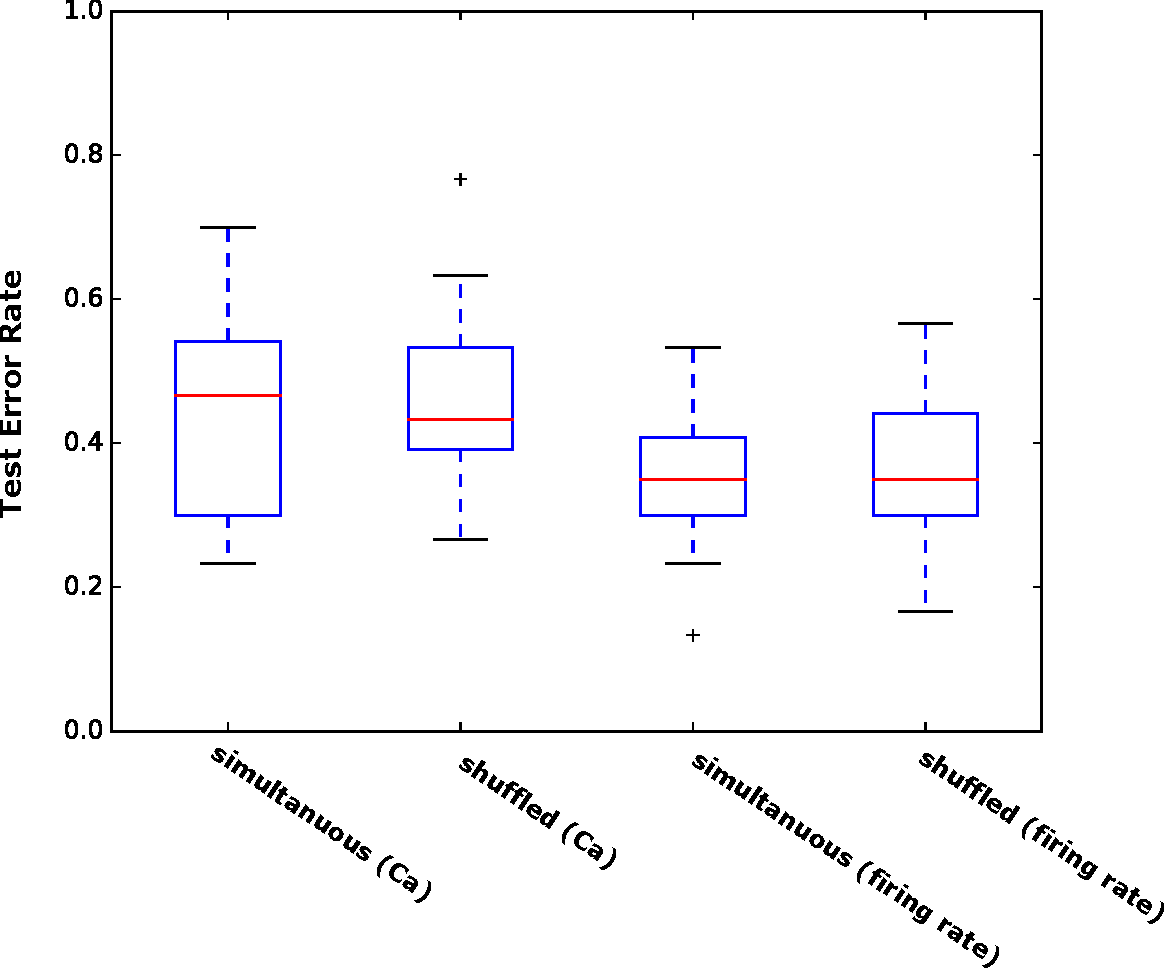
\includegraphics[scale=0.42]{sim_shf.pdf}
%\end{figure}
   \end{frame}
%________________________________________________________________________________
%____________________________________________________________________________________
\begin{frame}
\frametitle{\bf Decoding the Direction}
\begin{itemize}
\item SVM classifier for decoding direction of drifting gratings
\item Shuffled over different repeats of the stimulus. 
%\item Rotation invariant distance function
\end{itemize}
\visible{\begin{center}
\begin{tabular}{|c|c|cc}
\cline{1-2}
\multicolumn{2}{|c|}{stimuli}  & &\\
\hline
direction & tf (Hz) & \multicolumn{1}{c|}{cell\_1} & \multicolumn{1}{c|}{cell\_2}\\
\hline
$90\degree$ &  2 & \multicolumn{1}{c|}{\cellcolor{blue} 0} & \multicolumn{1}{c|}{\cellcolor{green} 0}\\
\hline
$90\degree$ &  2 & \multicolumn{1}{c|}{\cellcolor{green} 3} & \multicolumn{1}{c|}{\cellcolor{red} 2}\\
\hline
$90\degree$ &  2 & \multicolumn{1}{c|}{\cellcolor{yellow} 2} & \multicolumn{1}{c|}{\cellcolor{yellow} 2}\\
\hline
$90\degree$ &  2 & \multicolumn{1}{c|}{\cellcolor{red} 4} & \multicolumn{1}{c|}{\cellcolor{blue} 1}\\
\hline
\end{tabular}
\end{center}}
%
%\begin{figure}
%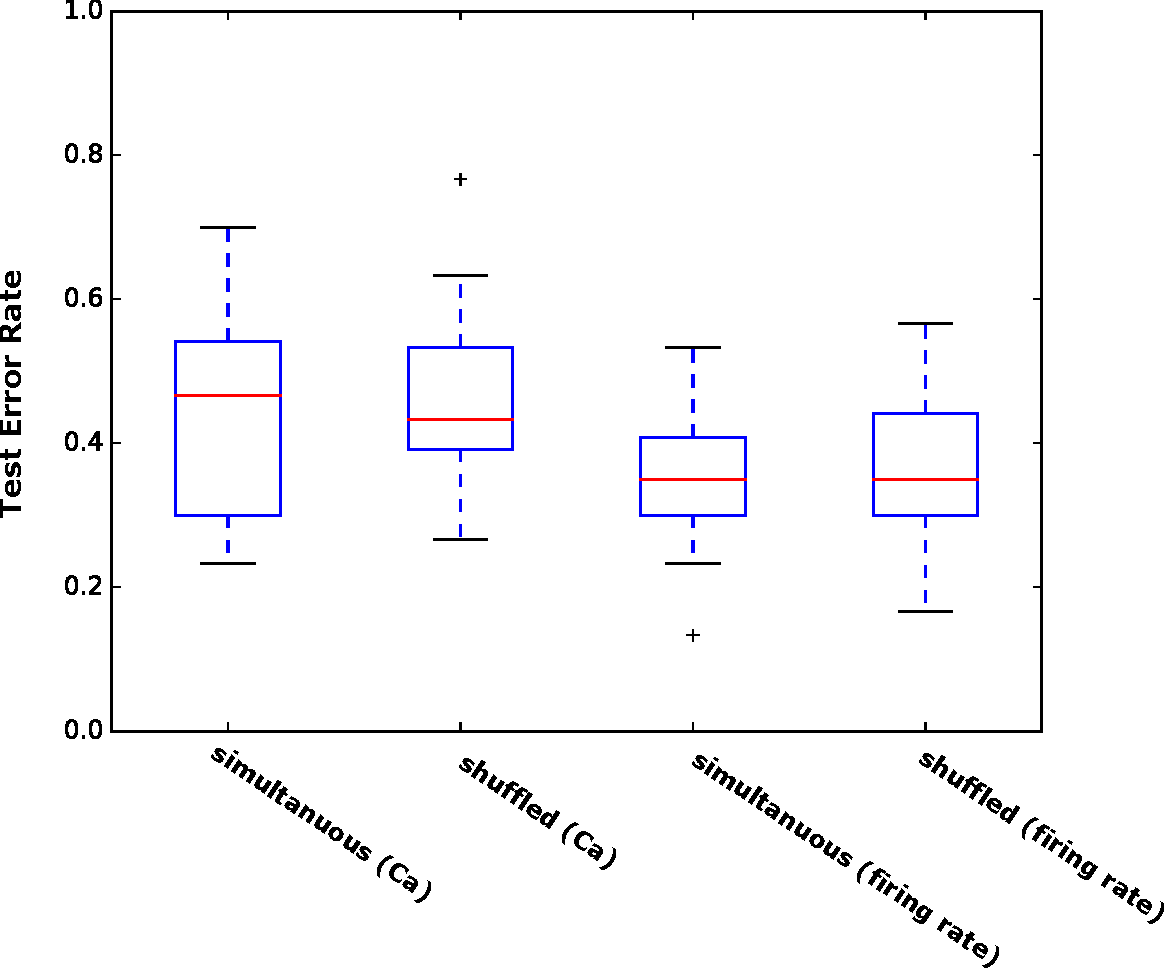
\includegraphics[scale=0.42]{sim_shf.pdf}
%\end{figure}
   \end{frame}
%________________________________________________________________________________
%____________________________________________________________________________________
\begin{frame}
\frametitle{\bf Decoding the Direction}
\begin{itemize}
\item Cre\_line:  Cux2-CreERT2, Imaging Depth = 275\pause
\item 8 labels are $\{0,45,90,135,180,225,270,315\}$\pause
\item \textbf{Chance performance:} $12.5 \%$\pause
\end{itemize}
\begin{figure}
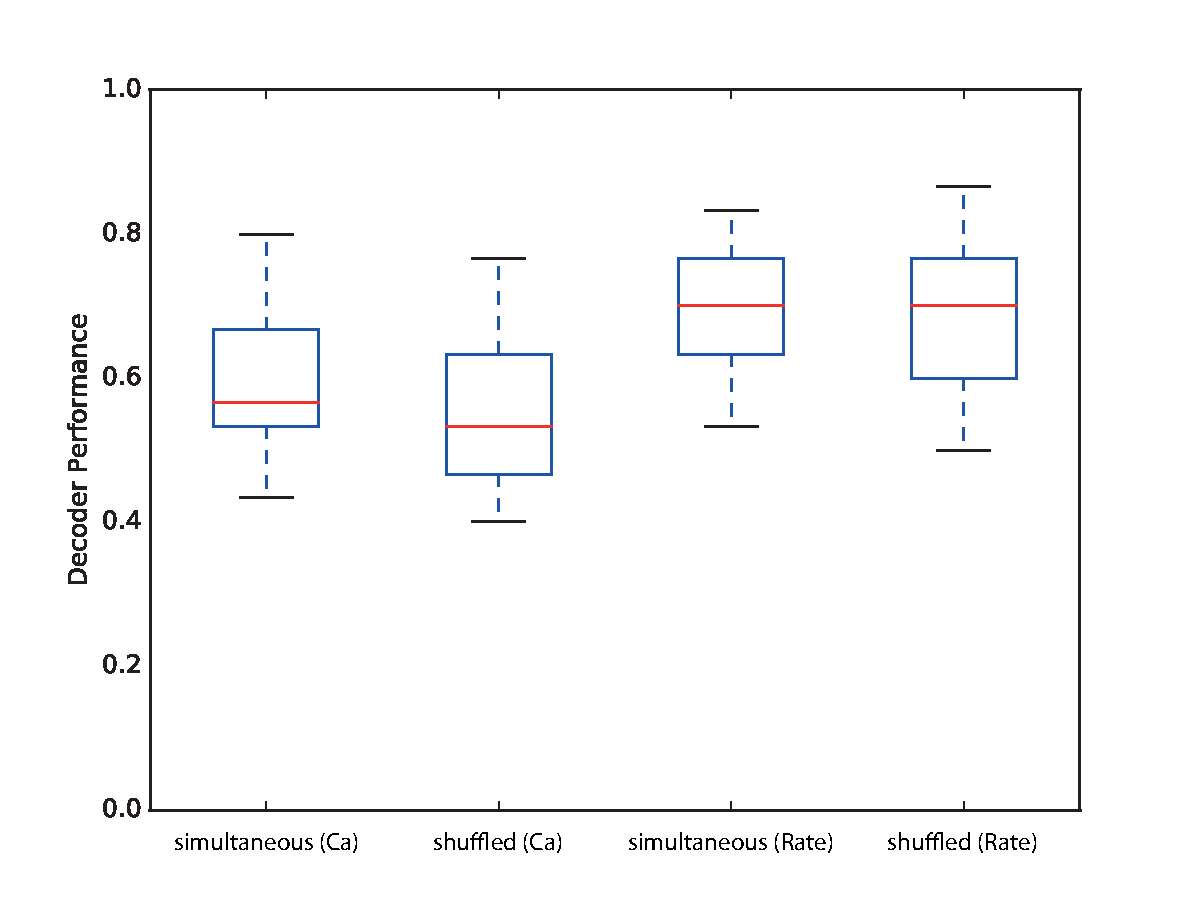
\includegraphics[scale=0.42]{sim_shf_p.pdf}
\end{figure}
   \end{frame}
%________________________________________________________________________________
%____________________________________________________________________________________
\begin{frame}
\frametitle{\bf Direction Selectivity Index}
\begin{gather*}
{\rm DSI} = \frac{R_{\rm pref} - R_{\rm null}}{R_{\rm pref} + R_{\rm null}}
\end{gather*}
\begin{figure}
 \begin{subfigure}{0.45\textwidth}
\centering    
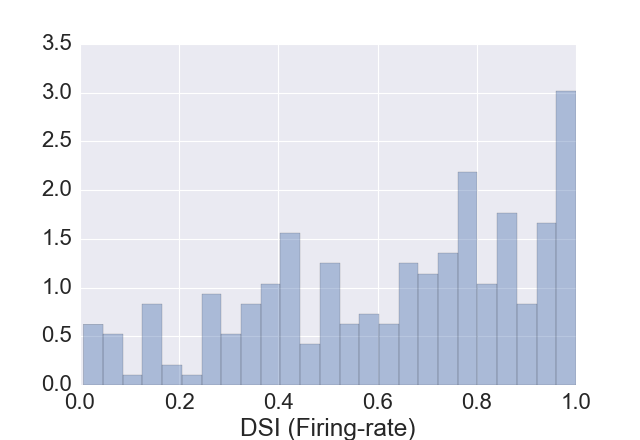
\includegraphics[scale=0.25]{DSI(Firing_rate).png}
 \end{subfigure}
 \begin{subfigure}{0.45\textwidth}
\centering    
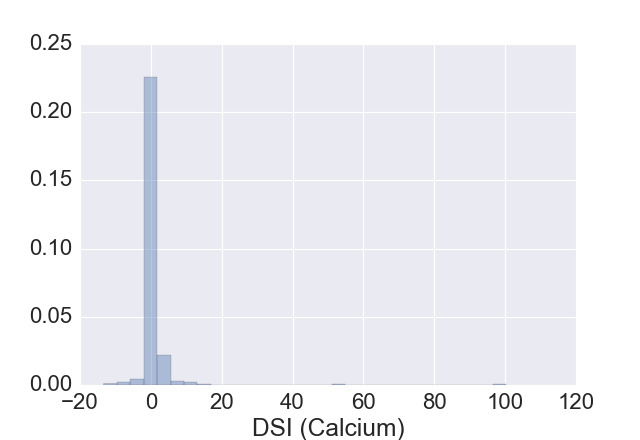
\includegraphics[scale=0.25]{DSI(Calcium).png}
            
 \end{subfigure}

\end{figure}
   \end{frame}
%________________________________________________________________________________


%____________________________________________________________________________________
\begin{frame}
%\frametitle{\bf Decoding the Direction}
\begin{itemize}
\item Use the $k$ cells with the largest DSI to decode direction.
\end{itemize}
\begin{figure}
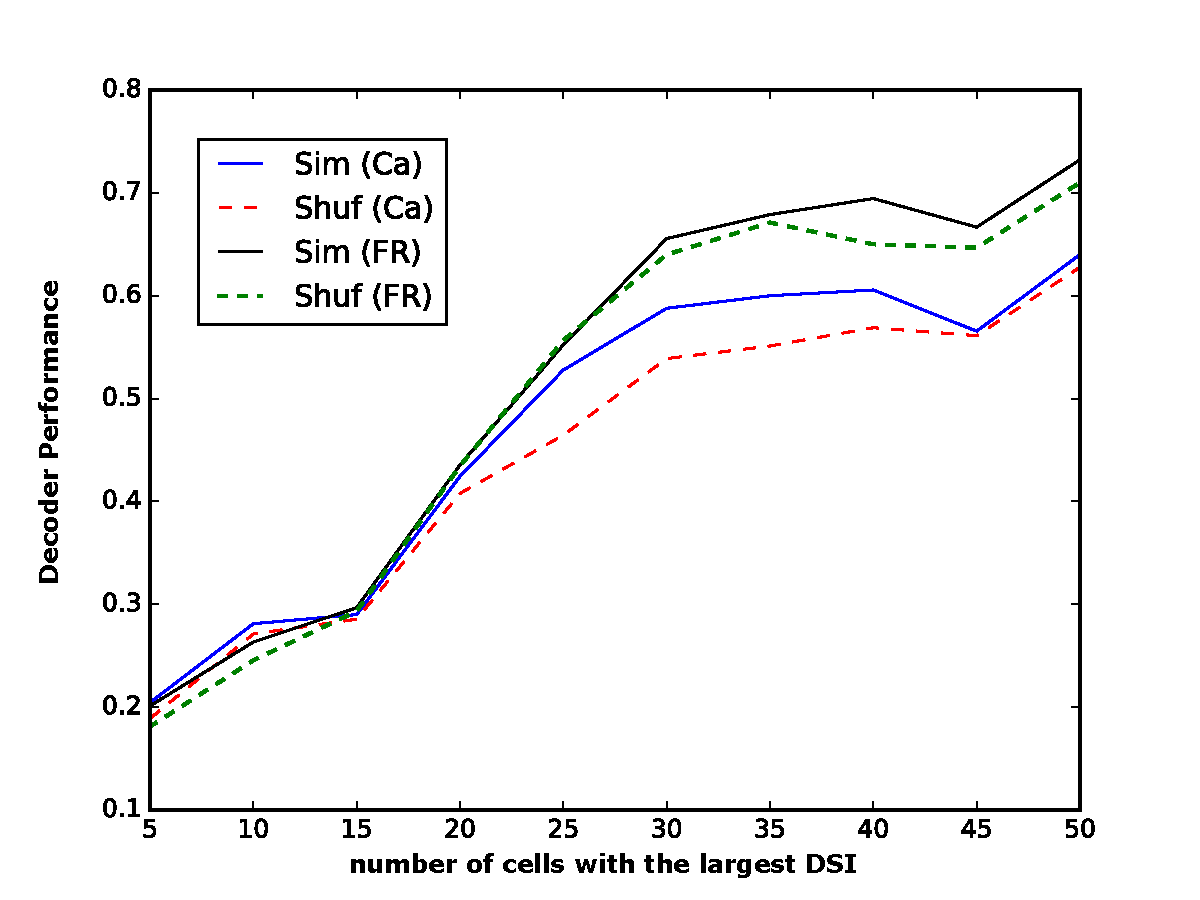
\includegraphics[scale=0.42]{best_r.pdf}
\end{figure}
   \end{frame}
%________________________________________________________________________________
%%________________________________________________________________________________


{
\setbeamercolor{background canvas}{bg=}
\includepdf[pages=7]{Anatoly_slides.pdf}
}


%____________________________________________________________________________________
\begin{frame}
\frametitle{\bf Linear Fisher Information}
\begin{figure}
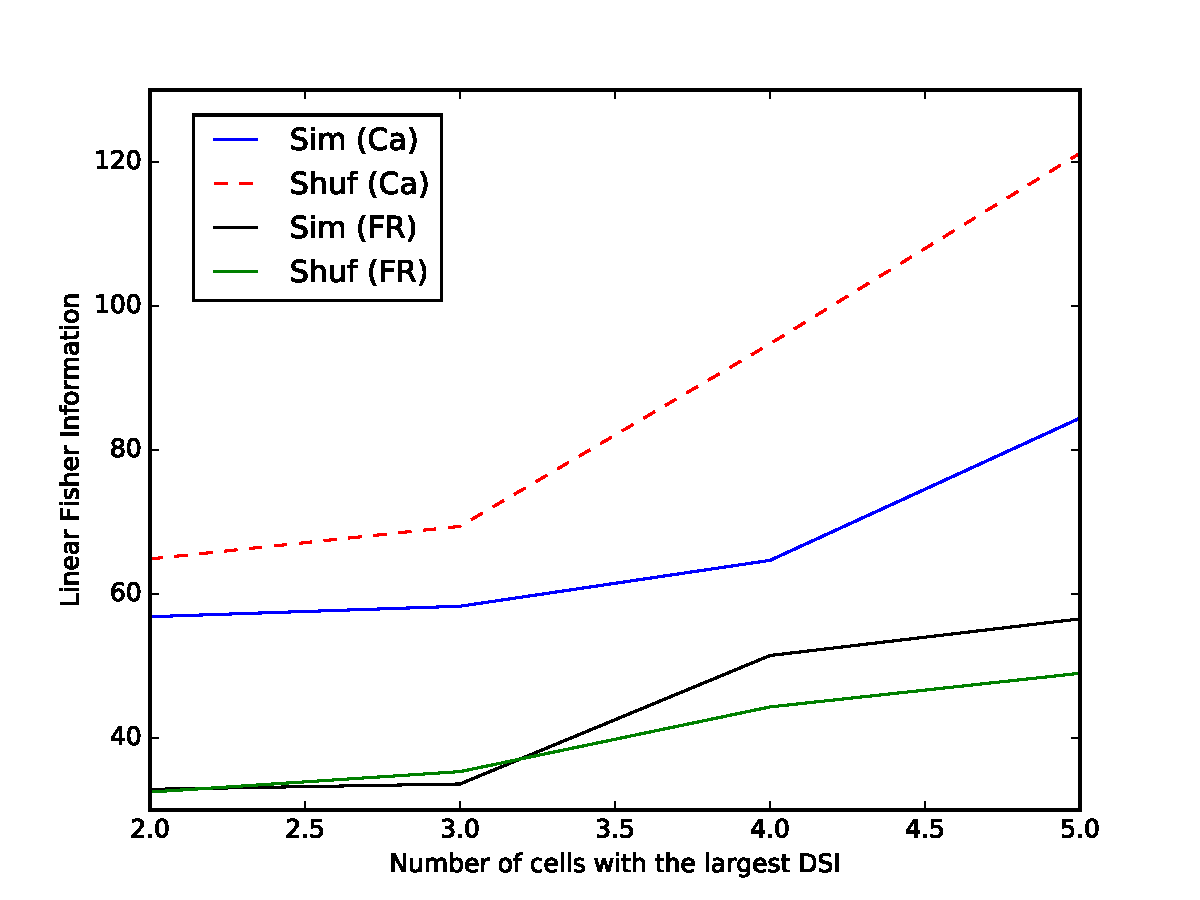
\includegraphics[scale=0.42]{fisher.pdf}
\end{figure}
   \end{frame}
%________________________________________________________________________________

%____________________________________________________________________________________
\begin{frame}
\frametitle{\bf Linear Fisher Information}
\begin{figure}
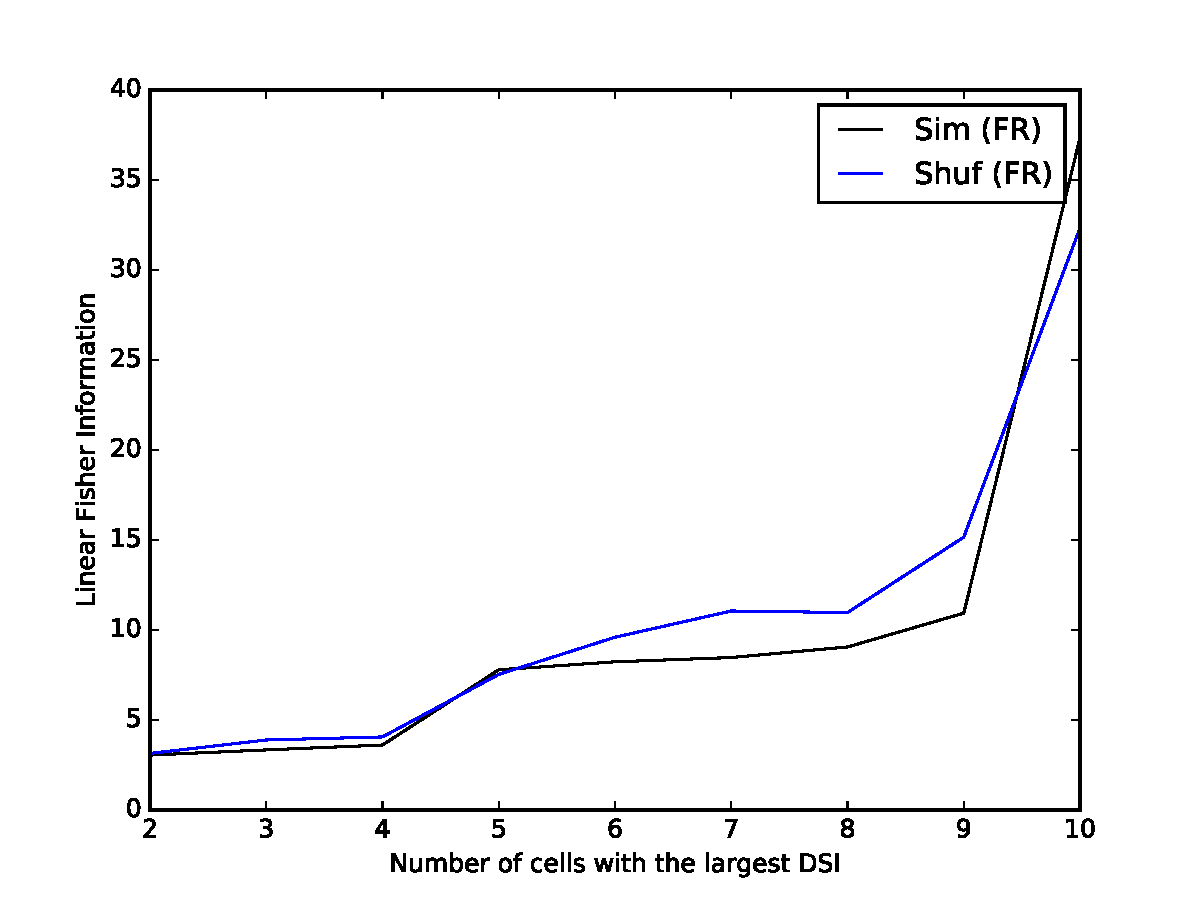
\includegraphics[scale=0.42]{fisher3.pdf}
\end{figure}
   \end{frame}
%________________________________________________________________________________

%\begin{frame}
%\frametitle{\bf Rotation Invariant Metric}
%
%Two neurons with shape preferences that are rotated version of each other should be close.\pause
%
%$$R(x,y) = \max_{\pi \in \Pi}{\rm corr}(x,\pi(y))$$
%
%$x,y$: normalized response of two cell to the set of shapes (366 dimensional vectors).
%
%$\Pi$ is the set, with elements corresponding to $8$ rotations. \pause
%
%$$d(x,y) = \frac{1}{2}(1- R(x,y))$$
%      \end{frame}
%%________________________________________________________________________________
%
%
%%________________________________________________________________________________
%\begin{frame}
%\frametitle{\bf Clusters}
%
%Six clusters were found with a density based clustering DBSCAN:
%
% The r-value Angular position and Curvature model (APC)
%\begin{figure}
%\includegraphics[scale=0.65]{figures/APC_r.png}
%\end{figure}
%
%
%
%      \end{frame}
%%________________________________________________________________________________
%
%
%%________________________________________________________________________________
%\begin{frame}
%\frametitle{\bf APC Models param.}
%
%
%Curvature mean and standard deviation
%\begin{figure}
%\includegraphics[scale=0.65]{figures/ap_sd.png}
%\end{figure}
%
%
%
%      \end{frame}
%%________________________________________________________________________________
%
%
% 
%%________________________________________________________________________________
%\begin{frame}
%\frametitle{\bf APC Models param.}
%
%
%Angular position mean and standard deviation
%\begin{figure}
%\includegraphics[scale=0.65]{figures/cr_sd.png}
%\end{figure}
%
%
%
%      \end{frame}
%%________________________________________________________________________________
%
% 
%   
%%________________________________________________________________________________
%\begin{frame}
%\frametitle{\bf Rotation invariance index}
%
%The index takes values in $[1, 8]$. $1$ indicates a perfect rotation invariant cell.
%\begin{figure}
%\includegraphics[scale=0.65]{figures/Rotation.png}
%\end{figure}
%
%
%
%      \end{frame}
%%________________________________________________________________________________
%
%
%%________________________________________________________________________________
%\begin{frame}
%\frametitle{\bf Tuning for Area}
%
%\begin{figure}
%\includegraphics[scale=0.65]{figures/cellsize.png}
%\end{figure}
%
%
%
%      \end{frame}
%%________________________________________________________________________________
%
%
%
%    %________________________________________________________________________________
%\begin{frame}
%\frametitle{\bf Summary of Clustering}
%\begin{center}
%  \begin{tabular}{ | l || r || r || r || r || r || r || r |}
%    \hline
%   &Total & Red & Blue & Yellow & Green & Purple  & Gray\\ \hline
%   Pasupathy & 109&  10 & 9 & 5 & 4& 3& 4\\ \hline 
%    Oleskiw  &    63  & 14 & 1 &0 &0 &0 & 0 \\ \hline
%   Popovkina  & 43&1   & 8  &1 &0 &3 & 0\\ \hline
%   Kosai        & 100&7    & 0  &3 &0 &0&1 \\ \hline
%   Sum        & 315&24    &31 &10&4&6&5 \\ \hline
%  \end{tabular}
%\end{center}
%
%
%
%      \end{frame}
%%________________________________________________________________________________
%
%
%   %________________________________________________________________________________
%\begin{frame}
%\frametitle{\bf Summary of Clustering}
%
%\frametitle{\bf Controls for Blue: Isoperimetric Quotient }
% 
% Measure of roundedness:  $\frac{4 \pi A}{L^2}$
%\begin{figure}
%\includegraphics[scale=0.65]{figures/isoq.png}
%\end{figure}
%
%
%      \end{frame}
%%______________
%
% 
%     %________________________________________________________________________________
%\begin{frame}
%\frametitle{\bf Summary of Clustering}
%
%\frametitle{\bf Controls for Blue: Isoperimetric Quotient }
% 
%Max response over $8$ rotations.
%\begin{figure}
%\includegraphics[scale=0.65]{figures/isoq51.png}
%\end{figure}
%
%
%      \end{frame}
%%______________

 

          

\end{document}